\label{chap:arch}

\begin{figure*}[ht] \centering
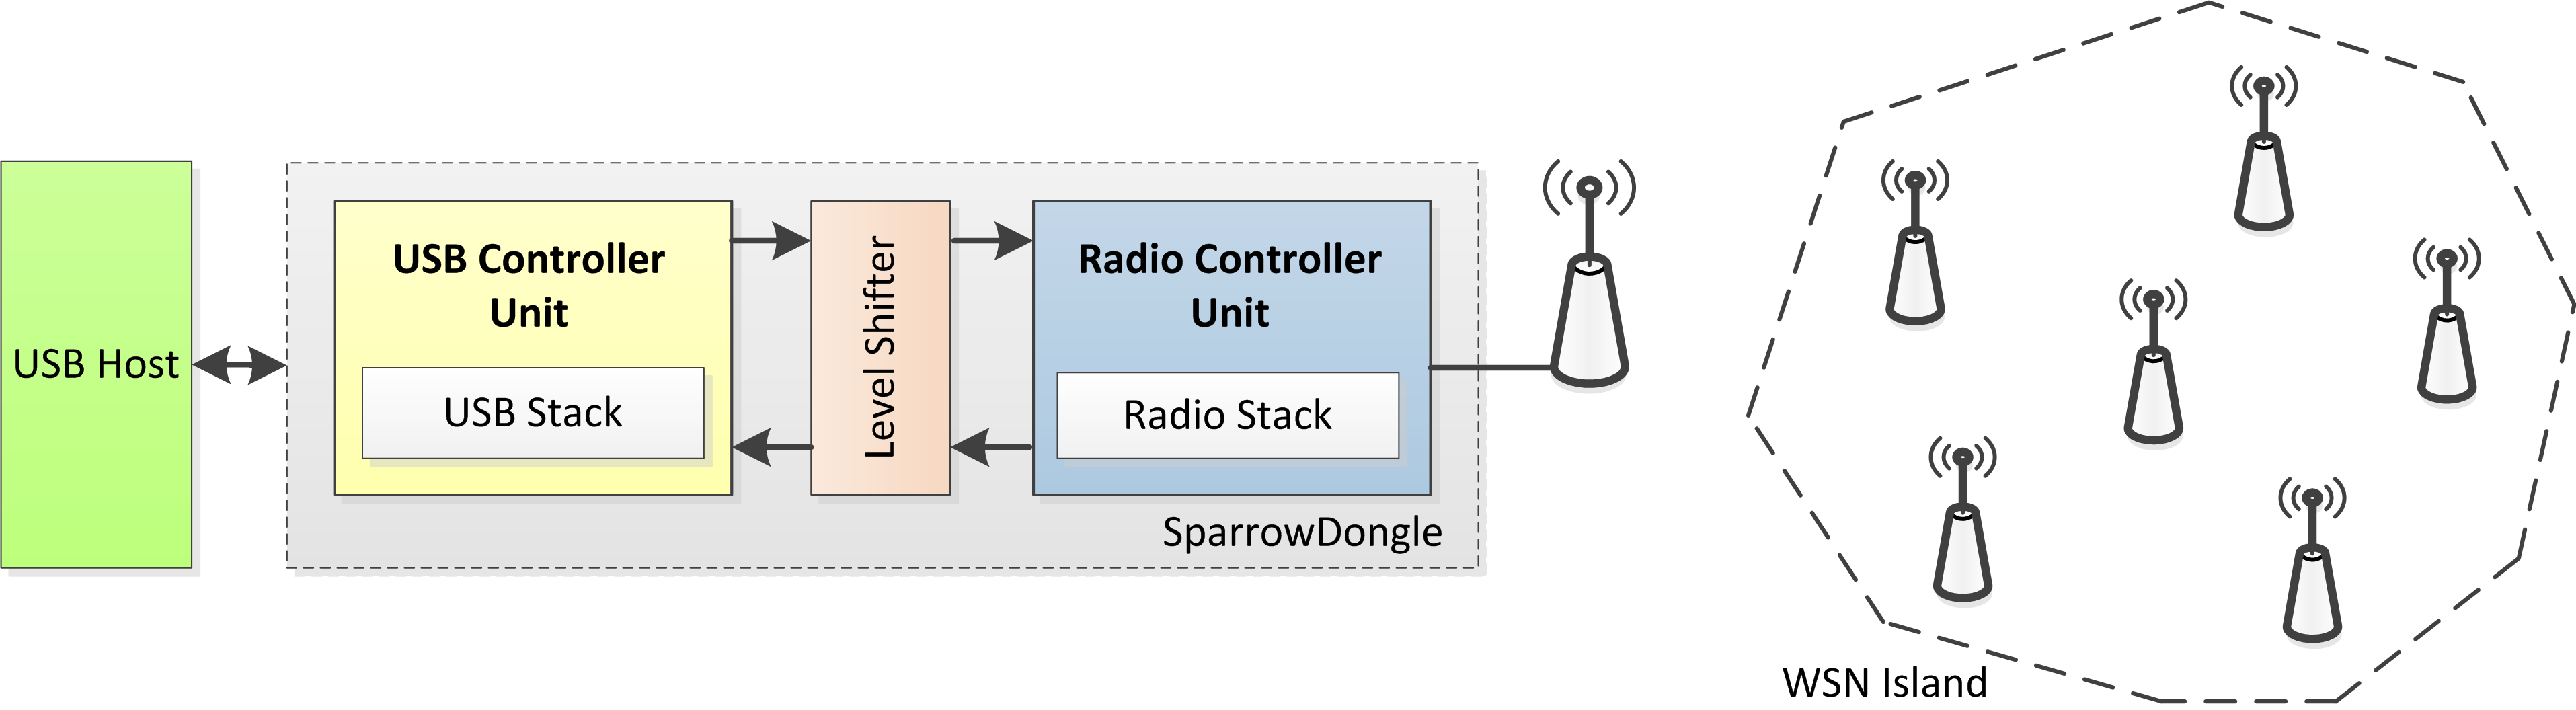
\includegraphics[width=0.9\textwidth]{img/Architecture.png}
\caption{SparrowDongle stick architecture} \end{figure*}

Te classic way of implementing a gateway is by using stationary devices or mobile devices like laptops or phones connected to at least one wireless node. The problem with this type of mobile devices is that you have to be in close proximity of the node in order to communicate with it. This might not be a problem if the nodes are easily accesible, but if a node is situated at a high altitude or over a clif, or even at an unknown location, using drones seems to be the best alternative.

Having this to say, our design has a number of features useful in everyday interaction with a wireless node outlined in \ref{sec:inter}. 

They can be launch from anyware, fly to any place a node might be placed and gather all the information collected by the nodes.

Additionally, a number of design features were included for ease-of-use in
research and development, outlined in \ref{sec:prox}


\subsection{\textit{Ease of interaction}} 

\label{sec:inter}

The drone automaticaly detects and initiates a comunication with a nearby node. It searches permanently for any signal emited by a node and sends an ack back to it when it receives any signal. After this first handshake is complet, the node has green light to transmit the information to the gateway installed on the drone. If a node has been detected, the pilot is informed of its presence and if the data transaction completed succesfuly so that he may continue in the search for another node.

\subsection{\textit{Proximity function}} 

\label{sec:prox}

The SparrowDongle can supply informations regarding the nearby nodes by reading the strength of the received signal. Using this information, the pilot can direct the drone closer to the nodes location, either for a faster transfer or to find its exact location. 

Besides the signal strength offered by the SparrowDongle, the drone features an onboard camera with a resolution of 1280x720 pixels streaming at 30 fps. This is very useful in determining the exact location of a wireless sensor node.


\ref{fig:progr}.


\begin{figure}[ht] \centering \label{fig:progr}
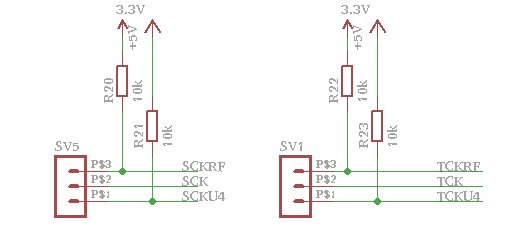
\includegraphics[width=0.35\textwidth]{img/progr.png} \caption{Header selection
for programming clock signals} \end{figure}



